\section{Como agregar un nuevo operador}

Para crear un nuevo operador se debe implementar la interfaz \textit{Operator} o alguna de sus subinterfaces o subclases. Esta interfaz cuenta con un �nico m�todo. La interfaz se muestra en la Figura \ref{fig:metaheuristics}. El m�todo de la interfaz es:
\begin{itemize}
    \item execute: M�todo que realiza una operaci�n sobre un operando y devuelve un objeto resultante de dicha operaci�n. Generalmente, este m�todo realiza una acci�n sobre una soluci�n o una lista de soluciones y retorna la soluci�n resultante de la operaci�n realizada.
\end{itemize}

Para configurar los par�metros del operador desde la ventana de configuraci�n, debe haber un constructor p�blico que posea la anotaci�n \textit{@DefaultConstructor}.

\subsection{\textit{@DefaultConstructor}}

La anotaci�n \textit{@DefaultConstructor} indica el constructor que debe ser usado al momento de crear una instancia del operador. Esta anotaci�n recibe un arreglo de \textit{NumberInput}, el cual se define en la siguiente secci�n. El arreglo debe tener la misma cantidad de argumentos que los par�metros del constructor como se muestra en la Figura \ref{fig:constructor_un_parametro} y Figura \ref{fig:constructor_multi_parametro}. 

\begin{figure}[H]
    \centering
    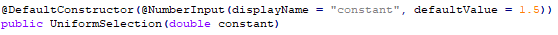
\includegraphics[width=\textwidth]{Seccion3/assets/ConstructorUnParametro.png}
    \caption{Constructor de un solo par�metro.}
    \label{fig:constructor_un_parametro}
\end{figure}
  
\begin{figure}[H]
    \centering
    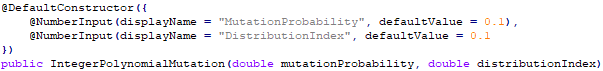
\includegraphics[width=\textwidth]{Seccion3/assets/ConstructorMultiParametro.png}
    \caption{Constructor de un solo par�metro.}
    \label{fig:constructor_multi_parametro}
\end{figure}

Esta anotaci�n solo puede ser usada en un �nico constructor por clase. Usar esta anotaci�n en m�s de un constructor lanzara una excepci�n en tiempo de ejecuci�n. Adicionalmente, el constructor que use esta anotaci�n solo puede tener par�metros de tipo \textit{int} o \textit{double}.

La interfaz gr�fica creada para cada anotaci�n se puede ver en la Figura \ref{fig:interfaz_uniform_selection} y \ref{fig:interfaz_polynomial_mutation}.

\begin{figure}[H]
    \centering
    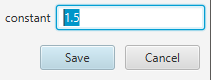
\includegraphics[width=0.5\textwidth]{Seccion3/assets/InterfazConfiguracionUniformSelection.png}
    \caption{Interfaz para configurar el operador \textit{UniformSelection}.}
    \label{fig:interfaz_uniform_selection}
\end{figure} 
 
\begin{figure}[H]
    \centering
    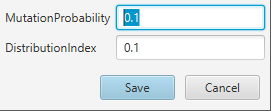
\includegraphics[width=0.5\textwidth]{Seccion3/assets/InterfazConfiguracionIntegerPolynomialMutation.png}
    \caption{Interfaz para configurar el operador \textit{IntegerPolynomialMutation}.}
    \label{fig:interfaz_polynomial_mutation}
\end{figure}

La anotaci�n puede tener un arreglo vac�o, lo cual indica que el constructor no recibir� par�metros.
